%% ---------------------------------------------------------------------
\section*{The firing squad in pictures}\phantomsection\label{sec:pictures}

Before the formal statement in \cref{sec:intro,sec:prelim}, here is the
problem as a story, in six pictures. The pictures of
\cref{fig:squad,fig:moods,fig:echo,fig:hare,fig:scoreboard} are drawings; the
configurations in \cref{fig:squad} and the diagrams of \cref{fig:squads14}
are computed by simulating the five-state rule $\delta_{14}$ of
\cref{tab:delta14}.

\paragraph{The squad}
A general stands at the left end of a line of $n$ soldiers
(\cref{fig:squad}). At time $0$ the general gives the order to fire, and
the order is: \emph{everybody fires at the same moment}. The difficulty is
that the soldiers are simple-minded. They are all alike, each of them can
only be in one of a few \emph{moods} (states), each of them only sees its
two neighbours (or the wall at the end of the line), and at every tick of a
common drum all of them change their moods at once, by looking up the
same rule book (\cref{fig:moods}). No soldier knows $n$, and none can count
to $n$: with five moods, a soldier can only tell five situations apart. Yet the rule book has to work for every length $n$.

\begin{figure}[htbp]
\centering
\begin{tikzpicture}[scale=0.93]
  \def\dx{0.82}
  % walls (the border) and rows
  \foreach \yy in {0,2.25,4.5} {\brickwall{0.30}{\yy}{1.3}\brickwall{7.02}{\yy}{1.3}}
  % t = 0: the general and seven sleeping soldiers
  \foreach \s [count=\i] in {G,L,L,L,L,L,L,L} {%
    \ifnum\i=1 \soldier{\i*\dx}{4.5}{\s}{shout}\else\soldier{\i*\dx}{4.5}{\s}{sleep}\zzz{\i*\dx}{4.5}\fi}
  % t = 4 (the configuration of delta_14 on 8 cells)
  \foreach \s [count=\i] in {L,A,B,B,B,L,L,L} {%
    \ifnum\i>5 \soldier{\i*\dx}{2.25}{\s}{sleep}\zzz{\i*\dx}{2.25}\else\soldier{\i*\dx}{2.25}{\s}{awake}\fi}
  % t = 14 = 2n-2: everybody fires
  \foreach \i in {1,...,8} {\soldier{\i*\dx}{0}{F}{fire}}
  % row labels
  \foreach \yy/\lab in {4.5/{$t=0$},2.25/{$t=4$},0/{$t=14$}}
    {\node[anchor=east,font=\small] at (0.25,\yy+0.65) {\lab};}
  % cell numbers
  \foreach \i in {1,...,8} {\node[font=\scriptsize,text=ink2] at (\i*\dx,4.33) {\i};}
  % the general's order
  \node[rectangle callout,draw=ink,fill=white,rounded corners=2pt,font=\sffamily\scriptsize,
        align=center,callout absolute pointer={(0.95,5.62)},inner sep=2pt] at (2.55,6.35)
        {All of you: fire at the same time!};
  % notes
  \begin{scope}[font=\scriptsize,text=ink,align=left,anchor=west,text width=3.75cm]
    \node at (7.55,5.15) {\textbf{Time 0.} The general $\mathsf G$ gives the
      order. Everybody else is quiescent ($\mathsf L$): asleep, and nobody
      knows how long the line is.};
    \node at (7.55,2.9) {\textbf{Every tick}, each soldier looks at its two
      neighbours (or the wall $\ast$) and changes its state by the same
      rule book. News travels at most one soldier per tick.};
    \node at (7.55,0.65) {\textbf{The goal.} Everybody fires ($\mathsf F$) at
      the same moment, and nobody earlier, for every length $n$. Best
      possible: $t=2n-2$, here $14$.};
  \end{scope}
  % ticking arrows
  \draw[-{Stealth[length=2mm]},ink2,line width=0.6pt] (-0.25,4.35) -- (-0.25,3.7);
  \draw[-{Stealth[length=2mm]},ink2,line width=0.6pt] (-0.25,2.1) -- (-0.25,1.45);
\end{tikzpicture}

\caption{A squad of $n=8$. Top: at time $0$ the general ($\mathsf G$)
gives the order and everybody else is quiescent ($\mathsf L$). Middle: at
time $4$ the news has reached cell $5$, and cells $6$ to $8$ are still
asleep. Bottom: at time $2n-2=14$ all soldiers fire together. The three
rows are the configurations of the rule $\delta_{14}$ on the line of length
$8$ at the times $0$, $4$ and $14$.}
\label{fig:squad}
\end{figure}

\begin{figure}[htbp]
\centering
\begin{tikzpicture}[scale=0.93]
  % the five moods
  \node[font=\small\bfseries,anchor=west] at (-0.2,2.05) {The five moods};
  \foreach \s/\f/\x/\lab in {L/sleep/0.3/asleep,G/shout/1.35/general,A/awake/2.4/helper,B/awake/3.45/helper,F/fire/4.5/fire!} {%
    \soldier{\x}{0}{\s}{\f}
    \node[font=\scriptsize,align=center,anchor=north] at (\x,-0.06) {$\mathsf{\s}$\\[-1pt]\lab};}
  \zzz{0.3}{0}
  % what one soldier sees
  \node[font=\small\bfseries,anchor=west] at (5.6,2.05) {One tick, one soldier};
  \soldier{6.05}{0}{G}{awake}
  \soldier{6.9}{0}{L}{awake}
  \soldier{7.75}{0}{L}{sleep}
  \draw[stG,line width=0.8pt,rounded corners=3pt,dashed] (5.72,-0.55) rectangle (8.08,1.62);
  \foreach \x/\lab in {6.05/left,6.9/me,7.75/right} {\node[font=\scriptsize,anchor=north] at (\x,-0.06) {\lab};}
  \draw[-{Stealth[length=2.2mm]},ink,line width=0.7pt] (8.3,0.7) -- node[above=2pt,font=\scriptsize]{next tick} (9.3,0.7);
  \soldier{9.6}{0}{A}{awake}
  \node[font=\scriptsize,anchor=north] at (9.6,-0.06) {me};
  % the rule book
  \node[draw=ink,fill=paper,rounded corners=2pt,anchor=north west,font=\scriptsize,align=left,
        inner sep=3pt] at (10.15,1.95) {%
      \textbf{rule book $\delta$}\\[1pt]
      $\mathsf L\,\mathsf L\,\mathsf L\to\mathsf L$\\
      $\mathsf G\,\mathsf L\,\mathsf L\to\mathsf A$\\
      $\mathsf L\,\mathsf G\,\mathsf L\to\mathsf A$\\
      $\mathsf G\,\mathsf G\,\mathsf G\to\mathsf F$\\[-2pt]
      \quad$\vdots$\\
      same book\\for everybody};
  \node[font=\scriptsize,text=ink,align=left,anchor=north west,text width=12.3cm] at (-0.2,-1.55)
    {With five states the book has $94$ free lines with $5$ possible entries
     each: $5^{94}\approx5\cdot10^{65}$ books. With four states there are
     $4^{43}\approx8\cdot10^{25}$ books, and none of them is a minimal-time
     solution (\cref{thm:four}). Is one of the five-state books a
     minimal-time solution? Nobody knows.};
\end{tikzpicture}

\caption{Left: the five states of a five-state rule. Right: one step of
one soldier. The soldier in the middle sees its left neighbour in state
$\mathsf G$, itself in state $\mathsf L$ and its right neighbour in state
$\mathsf L$, looks up the line $\mathsf G\,\mathsf L\,\mathsf L$ of the
rule book and becomes $\mathsf A$. The four lines shown are entries of
$\delta_{14}$ (\cref{tab:delta14}); the counts of rule books are those of
\cref{sec:five}.}
\label{fig:moods}
\end{figure}

\paragraph{Nobody can beat $2n-2$}
News travels at most one soldier per tick, so the soldier at the far end
wakes up at time $n-1$ at the earliest, and the fact that the line ends
there needs another $n-1$ ticks to travel back to the general: the general
cannot tell a squad of $6$ from a squad of $9$ before time $2\cdot6-2=10$
(\cref{fig:echo}). If the short squad fired earlier, the long squad would
see its general fire at the same time, long before its own right end has
even woken up. This is why $2n-2$ is the fastest possible firing time; a
rule book that achieves it for every $n$ is a \emph{minimal-time
solution}.

\begin{figure}[htbp]
\centering
\begin{tikzpicture}[scale=1]
  \def\u{0.36}\def\v{0.24}
  % two squads: n=6 at offset 0, n=9 at offset 3.1; agreement bound 2*6-2 = 10
  \foreach \n/\off in {6/0,9/3.1} {%
    \pgfmathtruncatemacro{\T}{2*\n-2}
    \foreach \t in {0,...,\T} {%
      \foreach \i in {1,...,\n} {%
        \pgfmathtruncatemacro{\s}{\t+\i}
        \pgfmathtruncatemacro{\lc}{\i-1}
        \pgfmathtruncatemacro{\rc}{2*\n-1}
        \ifnum\t<\lc \def\cc{white}\else
          \ifnum\t=\T \def\cc{stF}\else
            \ifnum\s=\rc \def\cc{stA}\else
              \ifnum\s>\rc \def\cc{refl}\else
                \ifnum\t=\lc \def\cc{stG}\else
                  \ifnum\s<11 \def\cc{agree}\else\def\cc{white}\fi
                \fi\fi\fi\fi\fi
        \filldraw[fill=\cc,draw=ink2!35,line width=0.2pt]
          (\off+\i*\u-\u,-\t*\v) rectangle (\off+\i*\u,-\t*\v-\v);
      }}
    \draw[ink,line width=0.6pt] (\off,0) rectangle (\off+\n*\u,-\T*\v-\v);
    % the anti-diagonal t+i = 10 | 11
    \draw[ink,densely dashed,line width=0.8pt] (\off,-11*\v) -- (\off+5.75*\u,-5.25*\v);
    \node[font=\small,anchor=south] at (\off+\n*\u/2,0.05) {$n=\n$};
  }
  % zzz in the quiet land of the long squad
  \node[font=\sffamily\bfseries\scriptsize,text=ink2] at (3.1+7.2*\u,-1.1*\v) {z z z};
  % labels
  \begin{scope}[font=\scriptsize,align=left]
    \node[anchor=west] (a) at (6.35,-0.4) {\textcolor{stG}{\rule{7pt}{7pt}} front: news moves one cell per tick};
    \node[anchor=west] at (6.35,-0.95) {\textcolor{stA}{\rule{7pt}{7pt}} echo from the wall (return chain)};
    \node[anchor=west] at (6.35,-1.5) {\textcolor{agree}{\rule{7pt}{7pt}} identical in both squads};
    \node[anchor=west] at (6.35,-2.05) {\textcolor{refl}{\rule{7pt}{7pt}} reflected triangle $R_n$};
    \node[anchor=west] at (6.35,-2.6) {\textcolor{stF}{\rule{7pt}{7pt}} everybody fires: $t=2n-2$};
    \node[anchor=north west,text width=4.6cm] at (6.3,-3.0) {Up to time $9$ the general (cell $1$)
      sees exactly the same in both squads. If the squad of $6$ fired
      earlier than $t=10$, the general of the squad of $9$ would fire too,
      long before its right end has even woken up. The echo needs $n-1$
      ticks to reach the wall and $n-1$ ticks to come back: no squad can
      beat $2n-2$.};
  \end{scope}
  \node[font=\scriptsize,anchor=east] at (-0.05,-0.12) {$t=0$};
  \node[font=\scriptsize,anchor=east] at (-0.05,-10.5*\v) {$t=10$};
  \node[font=\scriptsize,anchor=east] at (3.05,-16.5*\v) {$t=16$};
\end{tikzpicture}

\caption{Space-time diagrams (time runs downwards, one square per cell and
tick) of squads of $6$ and of $9$ soldiers, coloured by what each cell can
know. On the cells with $t+i\le10$ (light blue, bounded by the dashed
anti-diagonal) the two diagrams are equal cell by cell, for every rule
(\cref{lem:agree}); the right border can only
act in the reflected triangle, below the echo. The colours show regions,
not states.}
\label{fig:echo}
\end{figure}

\paragraph{Hare and tortoise}
How can a line of identical soldiers find its own middle? The classical
answer \cite{Minsky67} sends two messengers from the general: a hare
running at speed $1$ and a tortoise walking at speed $1/3$
(\cref{fig:hare}(a)). The hare bounces off the far wall at time $n-1$ and
meets the tortoise exactly in the middle, at time $3(n-1)/2$: the hare
has run $(n-1)+(n-1)/2$ cells when the tortoise has walked $(n-1)/2$. The
soldier in the middle becomes a new general for both halves, and the game
starts again, in both halves at once, until every piece is a single
soldier; everybody then fires after about $3n$ ticks. The minimal-time
solutions of Waksman and Balzer \cite{Waksman66,Balzer67} save time by
sending all the tortoises at once, at the speeds $1/3,1/7,1/15,\dots$
(\cref{fig:hare}(b)): the returning hare meets them at the points $n/2$,
$n/4$, $n/8,\dots$ at exactly the right times for all the pieces to finish
together at time $2n-2$. \Cref{thm:third,thm:left} say that some of this
is unavoidable in every minimal-time solution, whatever the number of
states: the non-periodic part of the diagram must reach the path of the
first tortoise, the line $i=t/3$, and the diagram cannot be periodic in any
wedge at the left border, where the slower and slower tortoises pile up.

\begin{figure}[htbp]
\centering
\begin{tikzpicture}[scale=1]
  % ---- (a) hare and tortoise: halving, about 3n (n = 17, one unit = one cell / one step)
  \begin{scope}[x=0.29cm,y=-0.095cm]
    \fill[paper] (0.5,0) rectangle (17.5,47);
    \draw[brick,line width=1.6pt] (0.5,0) -- (0.5,47) (17.5,0) -- (17.5,47);
    % level 1
    \draw[stG,line width=1.1pt] (1,0) -- (17,16) -- (9,24);
    \draw[stB,line width=1.1pt] (1,0) -- (9,24);
    % level 2
    \draw[stG,line width=0.8pt,dashed] (9,24) -- (17,32) -- (13,36) (9,24) -- (1,32) -- (5,36);
    \draw[stB,line width=0.8pt,dashed] (9,24) -- (13,36) (9,24) -- (5,36);
    % level 3
    \foreach \m/\d in {13/1,13/-1,5/1,5/-1} {%
      \draw[stG,line width=0.6pt,densely dotted] (\m,36) -- (\m+4*\d,40) -- (\m+2*\d,42);
      \draw[stB,line width=0.6pt,densely dotted] (\m,36) -- (\m+2*\d,42);}
    \foreach \p/\tt in {9/24,13/36,5/36,15/42,11/42,7/42,3/42} {\fill[flash,draw=ink,line width=0.3pt] (\p,\tt) circle (2.2pt);}
    \fill[stF] (0.5,45.5) rectangle (17.5,47);
    \node[font=\scriptsize,anchor=north] at (9,47.3) {everybody fires after about $3n$ ticks};
    \node[font=\small,anchor=south] at (9,-0.8) {(a) hare and tortoise};
    % icons: hare on the fast signal, tortoise on the slow one
    \begin{scope}[shift={(6.6,4.35)},x=1cm,y=1cm,scale=0.85]
      \fill[ink2!80] (0,0) ellipse (0.26 and 0.14);
      \fill[ink2!80] (0.25,0.12) circle (0.1);
      \fill[ink2!80,rotate around={62:(0.24,0.2)}] (0.24,0.42) ellipse (0.2 and 0.045);
      \fill[ink2!80,rotate around={48:(0.29,0.2)}] (0.29,0.42) ellipse (0.2 and 0.045);
      \fill[white] (0.29,0.14) circle (0.02);
      \fill[white,draw=ink2!80,line width=0.3pt] (-0.27,0.05) circle (0.06);
      \draw[ink2!80,line width=1pt,line cap=round] (0.12,-0.1) -- (0.25,-0.2) (-0.15,-0.1) -- (-0.3,-0.2);
    \end{scope}
    \begin{scope}[shift={(3.55,8.35)},x=1cm,y=1cm,scale=0.85]
      \fill[skin!60!ink2] (0.34,0.03) circle (0.075);
      \fill[skin!60!ink2] (-0.2,-0.03) rectangle (-0.12,-0.1) (0.12,-0.03) rectangle (0.2,-0.1);
      \filldraw[fill=stB!75!black,draw=ink,line width=0.3pt] (-0.29,-0.02) arc (180:0:0.29 and 0.22) -- cycle;
      \draw[stB!35,line width=0.4pt] (-0.1,-0.02) -- (-0.05,0.14) -- (0.07,0.14) -- (0.12,-0.02) (-0.05,0.14) -- (-0.14,0.19) (0.07,0.14) -- (0.14,0.19);
    \end{scope}
    \node[font=\scriptsize,anchor=west,stG!80!black] at (11.0,6.3) {hare, speed $1$};
    \node[font=\scriptsize,anchor=west,stB!70!black,align=left] at (0.75,19.0) {tortoise,\\speed $\tfrac13$};
    \node[font=\scriptsize,anchor=west,align=left] at (9.6,24.2) {they meet in\\the middle};
  \end{scope}
  % ---- (b) minimal time: all tortoises at once (n = 33)
  \begin{scope}[shift={(6.15,0)},x=0.165cm,y=-0.0735cm]
    \fill[paper] (0.5,0) rectangle (33.5,65);
    \draw[brick,line width=1.6pt] (0.5,0) -- (0.5,65) (33.5,0) -- (33.5,65);
    \draw[stG,line width=1.1pt] (1,0) -- (33,32) -- (1,64);
    \foreach \p/\tt in {17/48,9/56,5/60,3/62} {\draw[stB,line width=0.9pt] (1,0) -- (\p,\tt);
       \draw[ink2,densely dotted,line width=0.5pt] (\p,\tt) -- (\p,64);
       \fill[flash,draw=ink,line width=0.3pt] (\p,\tt) circle (2pt);}
    % the segment [17,33]: the same picture, mirrored, started by the wall
    \draw[stG,line width=0.7pt,dashed] (17,48) -- (33,64);
    \draw[stB,line width=0.7pt,dashed] (33,32) -- (25,56) (33,32) -- (29,60);
    \fill[flash,draw=ink,line width=0.3pt] (25,56) circle (1.6pt) (29,60) circle (1.6pt);
    \fill[stF] (0.5,64) rectangle (33.5,65.5);
    \node[font=\scriptsize,anchor=north] at (17,65.8) {everybody fires at $t=2n-2$};
    \node[font=\small,anchor=south] at (17,-1.1) {(b) all tortoises at once};
    \node[font=\scriptsize,anchor=west,align=left] at (12.5,14) {speeds $1,\tfrac13,\tfrac17,\tfrac1{15},\dots$};
    \node[font=\scriptsize,anchor=south] at (17,48.8) {$\tfrac n2$};
    \node[font=\scriptsize,anchor=south] at (9,56.5) {$\tfrac n4$};
    \node[font=\scriptsize,anchor=east,align=right] at (32.8,37.5) {echo};
  \end{scope}
\end{tikzpicture}

\caption{Space-time sketches of two classical constructions (time runs
downwards; walls in red). (a) Halving: the hare (speed $1$) and the tortoise
(speed $1/3$) meet in the middle; the construction is repeated in both
halves, here for $n=17$. (b) Minimal time, $n=33$: signals of speeds
$1/(2^j-1)$ meet the echo at $n/2$, $n/4$, $n/8,\dots$; each piece is
synchronized by a general at one of its ends, as shown with dashes for the
right half, and all pieces fire at $t=2n-2=64$.}
\label{fig:hare}
\end{figure}

\paragraph{How many moods?}
Each extra mood makes the rule book longer, and the question that has
occupied the field since the 1960s is: \emph{how few moods suffice for a
minimal-time solution?} Waksman needed $16$, Balzer $8$, Gerken $7$ and
Mazoyer $6$; with $4$ it is impossible (\cref{fig:scoreboard}). Five is the
one number nobody has settled. With five moods the rule book has $94$
free lines, so there are $5^{94}\approx5\cdot10^{65}$ books to choose
from, far too many to try one by one.

\begin{figure}[htbp]
\centering
\begin{tikzpicture}[scale=0.94]
  \draw[ink2,line width=0.8pt] (0.2,0) -- (11.4,0);
  \stone{4}{0.9}{ink2}{impossible}{Balzer 1967,\\Sanders 1994,\\certified here}
  \stone{5}{2.9}{stA}{\textbf{open}}{since 1987,\\this paper}
  \stone{6}{4.9}{stB}{solved}{Mazoyer\\1987}
  \stone{7}{6.7}{stB}{solved}{Gerken\\1987}
  \stone{8}{8.5}{stB}{solved}{Balzer\\1967}
  \stone{16}{10.8}{stB}{solved}{Waksman\\1966}
  \node[font=\small,text=ink2] at (9.65,0.02) {$\cdots$};
  \node[font=\scriptsize,anchor=east,align=right] at (0.5,0.75) {number of\\states $k$};
  % who is standing where
  \soldier{0.9}{0.32}{L}{sleep}
  \node[font=\bfseries\large,text=stA] at (1.35,1.75) {$\times$};
  \soldier{2.9}{0.32}{L}{awake}
  \node[ellipse callout,draw=ink,fill=white,font=\sffamily\bfseries\small,
        callout absolute pointer={(3.05,1.62)},inner sep=1pt] at (3.75,2.2) {?};
  \foreach \xx in {4.9,6.7,8.5,10.8} {\soldier{\xx}{0.32}{F}{fire}}
\end{tikzpicture}

\caption{The scoreboard of minimal-time solutions, by number of states
(references in \cref{sec:intro}). The four-state case is re-proved in
\cref{thm:four} with a certificate that is checked in six seconds; the
five-state case is the subject of this paper.}
\label{fig:scoreboard}
\end{figure}

\paragraph{So close}
We have not found a five-state solution, and we have not proved that
none exists. What we have found are five-state rule books that work for
every squad of at most $14$ soldiers. The best one, $\delta_{14}$, is shown
at work in \cref{fig:squads14}: with $14$ soldiers everybody fires at time
$26$, as required; with $15$ soldiers the three soldiers at the right end
fire at time $22$, six ticks too early. The rest of the paper explains why
such near misses are hard to rule out, and proves two general barriers that
every minimal-time solution must pass.

\begin{figure}[htbp]
\centering
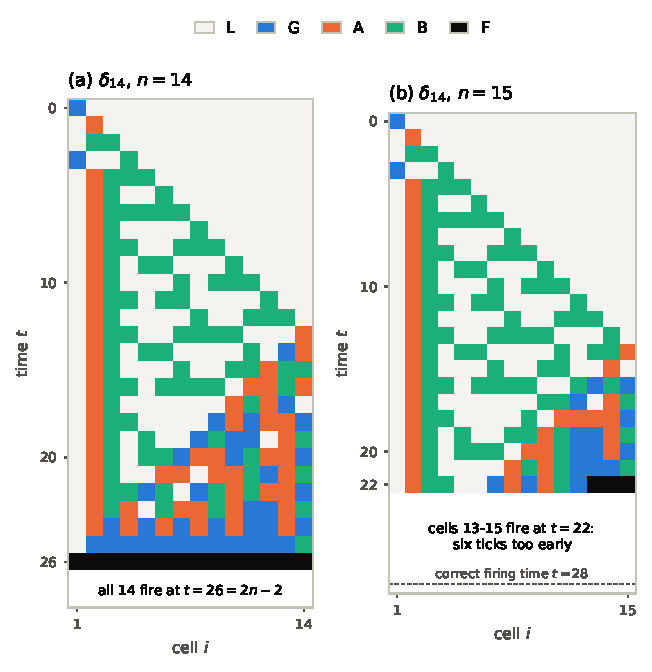
\includegraphics[width=0.64\textwidth]{fig_squads14.pdf}
\caption{The five-state rule $\delta_{14}$ (\cref{tab:delta14}) on squads
of $14$ and $15$ soldiers (time runs downwards, one square per cell and
tick, coloured by state). (a) All $14$ cells fire at $t=26=2n-2$. (b)
The cells $13$, $14$ and $15$ fire at $t=22$, before the correct firing
time $t=28$. Computed by direct simulation (\texttt{fsspcheck.c}).}
\label{fig:squads14}
\end{figure}

\FloatBarrier
